\documentclass[11pt,a4paper]{article}

\usepackage[utf8]{inputenc}
\usepackage[french]{babel}
\usepackage[T1]{fontenc}
\usepackage{graphicx}
\usepackage{listings}
\usepackage[hidelinks]{hyperref}
\usepackage{xcolor}
\usepackage{fancyhdr}
\usepackage{geometry}
\usepackage{float}
\usepackage{booktabs}
\usepackage{array}
\usepackage{amssymb}
\usepackage{enumitem}

\geometry{hmargin=2.3cm,vmargin=2.4cm}
\setlist{nosep,leftmargin=*}

\definecolor{codegray}{rgb}{0.5,0.5,0.5}
\definecolor{backcolour}{rgb}{0.95,0.95,0.92}
\definecolor{codegreen}{rgb}{0,0.5,0}

\lstset{
    language=Java,
    backgroundcolor=\color{backcolour},
    basicstyle=\ttfamily\footnotesize,
    breaklines=true,
    frame=single,
    keywordstyle=\color{blue},
    commentstyle=\color{codegreen},
    tabsize=2,
    showspaces=false, showstringspaces=false, showtabs=false,
    extendedchars=true,
    aboveskip=6pt, belowskip=6pt,
    literate={é}{{\'e}}1 {è}{{\`e}}1 {à}{{\`a}}1 {ç}{{\c{c}}}1 {ù}{{\`u}}1 {É}{{\'E}}1 {û}{{\^u}}1 {ê}{{\^e}}1 {î}{{\^i}}1 {ô}{{\^o}}1 {â}{{\^a}}1
}

\pagestyle{fancy}
\fancyhf{}
\lhead{TP 1 --- Analyse statique}
\rhead{HAI913I}
\cfoot{\thepage}
\renewcommand{\headrulewidth}{0.4pt}
\setlength{\headheight}{15pt}

\begin{document}

\begin{titlepage}
    \centering
    \begin{minipage}{0.45\textwidth}
        \begin{flushleft}
\includegraphics[width=2.3cm]{images/logo_mtp.png}\end{flushleft}
    \end{minipage}
    \hfill
    \begin{minipage}{0.45\textwidth}
        \begin{flushright}
\includegraphics[width=2.8cm]{images/faculte_science_logo.png}\end{flushright}
    \end{minipage}

    \vspace{2.5cm}
    \rule{\linewidth}{0.5pt}
    \vspace{0.4cm}

    {\huge \bfseries Rapport d'ingénierie \par}
    \vspace{0.4cm}
    {\Large \bfseries TP 1 : Analyse statique de programmes Java \par}
    \vspace{0.3cm}
    {\large HAI913I : Évolution et restructuration des logiciels \par}
    \rule{\linewidth}{0.5pt}

    \vspace{2.5cm}
    {\Large \textbf{SAMBARREY Adrien} \par}
    \vspace{0.1cm}
    {\large Numéro étudiant : 22510228 \par}
    \vspace{0.05cm}
    {\large Parcours GL \par}
    \vspace{0.7cm}
    {\Large \textbf{PREVOST-AVENEL Pierre} \par}
    \vspace{0.1cm}
    {\large Numéro étudiant : 22205821 \par}
    \vspace{0.05cm}
    {\large Parcours GL \par}

    \vspace{1.8cm}
    {\large Enseignant responsable : Bachar Rima \par}
    \vspace{0.2cm}
    {\large Année universitaire 2026--2027 \par}

    \vfill
    {\large Faculté des Sciences, Université de Montpellier \par}
    \vspace{0.3cm}
    {\large \today \par}
\end{titlepage}

\tableofcontents
\vspace{0.8cm}

\noindent\textbf{Résumé.} Cet analyseur statique lit les sources d'un projet Java avec Eclipse JDT Core, en extrait la structure et les appels, les range dans un modèle de faits qui ne doit rien à la bibliothèque d'analyse, et calcule sur ce seul modèle treize métriques et un graphe d'appel interrogeable dans les deux sens. Tous les points de contrôle du sujet sont franchis sans écart sur le projet de validation ; un projet tiers a été analysé en plus, et c'est lui qui a révélé le seul écart de comptage que nous rapportons. Les trois bonus sont traités : C1 (extraction Spoon), C2 (visualisation Graphviz et interface graphique) et C3 (analyse d'un projet de taille moyenne).

\newpage

\section{Objectifs et périmètre}

L'outil prend le chemin d'un projet Java et produit quatre familles de résultats : la structure, les appels de méthodes avec le type statique du receveur, treize métriques, et le graphe d'appel interrogeable dans les deux sens.

\textbf{Constructions prises en charge} (Java 17) : classes, interfaces, énumérations, \textit{records}, classes membres ; classes anonymes et locales reconnues mais exclues du comptage (§4.1) ; lambdas, dont les appels sont attribués à la méthode englobante ; héritage vers les classes de bibliothèque ; génériques désignés par leur effacement.

\textbf{Ce que l'outil ne fait pas}, par choix et conformément au sujet : aucune expansion des appels virtuels (ni CHA ni RTA), aucune prise en compte de la réflexion, des proxys ou de l'injection de dépendances, aucun arc vers les constructeurs (qui restent des n\oe{}uds). L'analyse répond à « $f$ nomme-t-elle $g$ dans son code ? », pas à « $f$ appellera-t-elle $g$ à l'exécution » ; les conséquences sont discutées en section \ref{sec:critique}.

\section{Conception générale}

\subsection{La frontière autour de JDT}

Nous avons suivi la recommandation de l'annexe 1 : \textbf{aucun traitement ne manipule un type JDT}. \texttt{parse} et \texttt{extract} sont les seuls paquetages à travailler sur l'AST, \texttt{spoon} (bonus C1) sur son équivalent Spoon.

Décompte des imports sur l'ensemble de \texttt{src/main} :

\begin{lstlisting}[language=bash]
$ grep -rc "^import org.eclipse" src/main/java/hai913i/tp1/ | grep -v ":0$"
cli/Analyzer.java:1
parse/JdtParser.java:5
extract/StructureVisitor.java:15
extract/AstPrinter.java:2
extract/CallCollector.java:11
\end{lstlisting}

\texttt{model}, \texttt{metrics}, \texttt{callgraph} et \texttt{report} n'apparaissent pas dans la liste : l'exigence B1 est tenue là où elle porte, sur les traitements.

L'import de \texttt{cli/Analyzer.java} est le seul en dehors de \texttt{parse} et \texttt{extract}. Il s'agit d'\texttt{IProblem}, utilisé pour afficher les erreurs de compilation remontées par le parseur. \texttt{Analyzer} enchaîne les composants et ne calcule rien, ce qui rend l'import sans conséquence sur les résultats, mais la frontière est imparfaite à cet endroit. Faire remonter les diagnostics sous la forme d'un \textit{record} maison suffirait à la fermer ; nous ne l'avons pas fait.

Trois conséquences pratiques, constatées après coup : l'extraction Spoon s'est branchée sur le même modèle sans qu'une ligne de traitement change ; la règle des « 10 \% » se teste sur des données écrites à la main, sans lancer d'analyse ; l'interface graphique et l'export DOT ne recalculent rien.

\subsection{Représentation des faits}

Le modèle tient en cinq \texttt{record} immuables. \texttt{ProjectFacts} rassemble le tout ; \texttt{TypeFact} porte le nom qualifié, le paquetage, le genre, les superclasses, les interfaces, les attributs et les méthodes ; \texttt{FieldFact} décrit un attribut ; \texttt{MethodFact} retient l'identifiant, le nom, les types des paramètres, le caractère de constructeur, la visibilité, les lignes du corps et les appels ; \texttt{CallFact} enfin décrit un appel par son appelant, le nom appelé, la cible, le receveur statique, la ligne, et deux drapeaux, résolu et interne.

Une méthode est désignée par une chaîne de la forme \texttt{library.service.Catalog\#add(library.model.Item)}, jamais par un objet JDT. Les types des paramètres en font partie, ce qui suffit à faire de deux surcharges deux n\oe{}uds distincts ; ils sont donnés par leur effacement, comme l'impose le §4.4. L'identifiant ne dépend donc pas de la bibliothèque qui l'a produit : le graphe construit à partir de Spoon est le même que celui construit à partir de JDT, et la comparaison du bonus C1 se ramène à confronter les compteurs deux à deux.

Classes imbriquées : \texttt{LoanService.Loan} est un type à part entière avec ses 4 méthodes, et \texttt{LoanService} n'en garde que 6. Les membres sont lus par \texttt{bodyDeclarations()}. Une visite récursive, plus naturelle à écrire, aurait fait remonter les méthodes de \texttt{Loan} dans \texttt{LoanService} sans rien signaler.

Les appels non résolus, eux, sont conservés comme des faits à part entière, avec \texttt{resolved} à faux et un \texttt{targetId} vide : ils sont comptés et affichés, mais ne produisent aucun arc. Il n'y en a aucun sur le projet de validation et un seul sur \texttt{missing-dep}. Quant au déterminisme exigé par B1, il repose sur trois tris explicites et rien d'autre : les fichiers par chemin, les types par nom qualifié, les arcs par \texttt{TreeMap}.

\section{Réponses étape par étape}

\subsection{A0 --- Environnement et lecture du projet}

\texttt{ProjectSources} ne fait aucune analyse : il répond à « où est la racine des sources » (\texttt{src/main/java}, sinon \texttt{src}, sinon le projet) et « quels \texttt{.java} contient-elle ». \texttt{JdtParser} est la seule classe qui connaît la configuration d'\texttt{ASTParser} : c'est une façade.

\begin{table}[H]
\centering\small
\begin{tabular}{@{}p{4.3cm}p{4.1cm}p{6cm}@{}}
\toprule
\textbf{Réglage} & \textbf{Rôle} & \textbf{Si on l'enlève} \\
\midrule
\texttt{setResolveBindings(true)} & calculer les \textit{bindings} & \textbf{0/93} résolu \\
\texttt{setEnvironment(...)} & où chercher les types & \texttt{IllegalStateException: Missing system library} \\
4\textsuperscript{e} argument à \texttt{true} & inclure le JDK courant & même exception \\
\texttt{setComplianceOptions(17)} & niveau du code analysé & un \texttt{record} est lu comme du Java 25 \\
\texttt{createASTs} en un seul lot & résolution partagée & les appels entre fichiers ne se résolvent plus \\
racine $=$ \texttt{src}, pas le projet & résolution des paquetages & \textbf{49/93}, \textit{sans aucune erreur} \\
\bottomrule
\end{tabular}
\end{table}

La dernière ligne est une \textbf{panne silencieuse} : aucune exception, simplement la moitié des appels qui cessent d'être résolus.

\textbf{Résultat} : 14 unités de compilation, 0 erreur. Comme \texttt{setBindingsRecovery(true)} masque beaucoup de choses, nous avons ajouté une vérification explicite : \textbf{93 \texttt{MethodInvocation}, 93 résolus, 0 \textit{binding} nul}, ce qui correspond à la variante A mesurée dans l'annexe 2.

\subsection{A1 --- Parcourir un AST}

\texttt{AstPrinter} utilise les deux crochets appelés sur \textbf{tous} les n\oe{}uds, avec un compteur de profondeur, plutôt que de redéfinir les quelque quatre-vingt-dix méthodes \texttt{visit} de l'API.

\begin{lstlisting}
@Override public boolean preVisit2(ASTNode node) {
    System.out.println("  ".repeat(depth) + node.getClass().getSimpleName());
    depth++;
    return true;
}
@Override public void postVisit(ASTNode node) { depth--; }
\end{lstlisting}

Sur \texttt{Dvd.java}, le point de contrôle est atteint : un \texttt{TypeDeclaration}, un \texttt{FieldDeclaration} et trois \texttt{MethodDeclaration} dont le constructeur contenant un \texttt{SuperConstructorInvocation}. Trois observations ont servi à A2 : le \texttt{FieldDeclaration} et son \texttt{VariableDeclarationFragment} sont deux n\oe{}uds distincts, et c'est le fragment qu'il faut compter ; le constructeur est un \texttt{MethodDeclaration} ordinaire, seul \texttt{isConstructor()} le distingue ; la Javadoc est un enfant de la \texttt{MethodDeclaration}, d'où le piège des positions.

Sur \texttt{Category.java}, la racine du type est un \textbf{\texttt{EnumDeclaration}}, qui n'hérite pas de \texttt{TypeDeclaration} : les deux descendent d'\texttt{AbstractTypeDeclaration}. Un visiteur ne redéfinissant que \texttt{visit(TypeDeclaration)} compterait \textbf{14 types au lieu de 15}. Les \texttt{EnumConstantDeclaration} n'étant pas des \texttt{FieldDeclaration}, l'exclusion des constantes d'énumération du §4.1 est gratuite avec JDT, contrairement à Spoon (section \ref{sec:bonus}).

\subsubsection*{Rôle de la valeur renvoyée par \texttt{visit(...)}}

Le parcours est en profondeur, piloté par \texttt{accept}. Pour chaque n\oe{}ud, JDT appelle \texttt{preVisit2}, puis le \texttt{visit} de son \textbf{type concret} : c'est une double répartition, le n\oe{}ud connaît sa classe et le visiteur sait quoi faire, sans aucun test de type dans notre code. \textbf{La valeur renvoyée décide si les enfants sont visités} : \texttt{true} fait descendre, \texttt{false} élague le sous-arbre, le n\oe{}ud ayant tout de même été vu. \texttt{endVisit} et \texttt{postVisit} ne renvoient rien, puisqu'à la remontée il n'y a plus de décision à prendre.

Vérifié expérimentalement : avec \texttt{visit(MethodDeclaration)} renvoyant \texttt{false} sur \texttt{Dvd.java}, les trois méthodes apparaissent toujours mais vides, sans \texttt{Block} ni \texttt{ReturnStatement}.

Dans notre outil, \texttt{return false} sur une \texttt{AnonymousClassDeclaration} réalise en une ligne la règle « les classes anonymes ne comptent pas ». \textbf{Limite} : cet élagage vaut pour les \textit{types}, pas pour les \textit{appels}, que le §4.4 attribue à la méthode englobante. Réutiliser le même visiteur pour A2 et A3 nous aurait fait perdre l'appel \texttt{item.isAvailable()} de \texttt{Catalog.available}.

\subsection{A2 --- Extraire la structure}

\texttt{StructureVisitor} redéfinit trois \texttt{visit}, un par sorte de déclaration de type, et lit les membres par \texttt{bodyDeclarations()}.

\begin{lstlisting}
@Override public boolean visit(TypeDeclaration node) {
    if (node.isLocalTypeDeclaration()) return false;   // classe locale : non comptee
    record(node, node.isInterface() ? TypeKind.INTERFACE : TypeKind.CLASS);
    return true;                     // on descend : les types membres comptent
}
@Override public boolean visit(EnumDeclaration node)   { record(node, TypeKind.ENUM);   return true; }
@Override public boolean visit(RecordDeclaration node) { record(node, TypeKind.RECORD); return true; }
@Override public boolean visit(AnonymousClassDeclaration node) { return false; }
\end{lstlisting}

Le \texttt{return true} laisse le parcours atteindre les types membres comme \texttt{LoanService.Loan} ; combiné à la lecture par \texttt{bodyDeclarations()}, il produit le comptage attendu.

\textbf{Conventions retenues} : comptage des \texttt{fragments()}, car \texttt{int a, b;} vaut deux attributs ; superclasses obtenues par \texttt{getSuperclass()} en boucle jusqu'avant \texttt{java.lang.Object}, l'AST ne donnant que la superclasse directe ; \texttt{getErasure()} sur tous les noms de types ; visibilité par défaut \texttt{PACKAGE}, sauf membre d'interface qui est \texttt{PUBLIC} implicite ; lignes mesurées sur \texttt{getBody()} et non sur la \texttt{MethodDeclaration}, dont la position commence à la Javadoc, avec \texttt{getLineNumber(start + length - 1)} pour la dernière ligne.

\textbf{Résultat} : 15 types, 59 méthodes dont 9 constructeurs, 21 attributs, 4 paquetages. Les vérifications détaillées passent également : \texttt{LoanService} 6 méthodes et 5 attributs, \texttt{LoanService.Loan} 4 et 3 comptés à part, superclasses de \texttt{LoanException} égales à \texttt{[Exception, Throwable]}, cinq visibilités de \texttt{Item} conformes.

\subsection{A3 --- Appels et type statique du receveur}

\texttt{CallCollector} est lancé sur le \textbf{corps} de chaque méthode comptée, et non sur le fichier : ce choix rattache chaque appel à sa méthode englobante et écarte gratuitement les appels hors de toute méthode. Deux \texttt{visit} seulement, \texttt{MethodInvocation} et \texttt{SuperMethodInvocation} ; oublier le second donne 93 appels au lieu de 94. Les références de méthode \texttt{T::m} ne sont pas des appels. Aucun élagage des lambdas ni des classes anonymes, contrairement à \texttt{StructureVisitor}.

\begin{lstlisting}
private String receiverOf(MethodInvocation node, IMethodBinding target) {
    Expression receiver = node.getExpression();
    if (receiver != null) return nameOf(receiver.resolveTypeBinding());  // type declare
    if (target != null && Modifier.isStatic(target.getModifiers()))
        return nameOf(target.getDeclaringClass());        // import statique compris
    return nameOf(enclosingTypeOf(node));                 // this implicite
}
\end{lstlisting}

Pour \texttt{super.m()}, la règle diffère : le receveur est la superclasse directe du type englobant.

\textbf{Résultat} : 94 appels, 46 internes, 48 externes, 0 non résolu. Les quatre cas particuliers sont conformes : receveur \texttt{Loanable} et non \texttt{Item} pour \texttt{loanable.checkOut()} ; receveur \texttt{Book} mais cible héritée \texttt{Item\#getTitle()} ; receveur \texttt{Item} pour le \texttt{super.describe()} de \texttt{Book} ; appel capté dans la lambda de \texttt{Catalog.available}.

Le troisième cas est le plus utile à vérifier : sur la \textbf{même ligne 32} de deux fichiers, \texttt{dune.describe()} donne un receveur \texttt{Book} et \texttt{super.describe()} un receveur \texttt{Item}. Les deux règles sont donc bien appliquées séparément.

\subsection{B1 --- Un modèle de faits indépendant de JDT}

Le modèle ayant été construit au fil de A2 et A3, cette étape a consisté à vérifier trois propriétés : l'indépendance vis-à-vis de JDT (section 2), le fait que tous les chiffres de A2 et A3 soient recalculés depuis le seul modèle par des méthodes de \texttt{ProjectFacts}, et le déterminisme, deux exécutions comparées par \texttt{diff} donnant des sorties identiques.

\subsection{B2 --- Métriques}

Les questions 8, 9 et 12 reposent sur la même règle, isolée dans \texttt{Ranking} et testée séparément.

\begin{lstlisting}
/** Plafond de n/10 en entiers. (int) (n * 0.1) arrondirait vers le bas. */
public static int quota(int candidateCount) { return (candidateCount + 9) / 10; }

public static <T> List<T> topTenPercent(List<T> candidates,
        ToIntFunction<T> value, Function<T, String> name) {
    if (candidates.isEmpty()) return List.of();
    List<T> sorted = candidates.stream()
            .sorted(Comparator.comparingInt(value).reversed().thenComparing(name)).toList();
    int cut = value.applyAsInt(sorted.get(quota(candidates.size()) - 1));
    return sorted.stream().filter(c -> value.applyAsInt(c) >= cut)
                          .filter(c -> value.applyAsInt(c) > 0).toList();
}
\end{lstlisting}

Trois clauses sont des pièges. $k = \lceil n/10 \rceil$ calculé par \texttt{(n + 9) / 10} : le transtypage \texttt{(int) (n * 0.1)} donnerait 1 au lieu de 2 pour $n = 15$. Les ex \ae{}quo du $k$-ième sont retenus, donc le résultat peut dépasser $k$ : question 8, $k = 2$ mais \texttt{Member} et \texttt{LoanService} sont à égalité à 6 méthodes, d'où trois classes. Une valeur nulle n'est jamais retenue, même dans les $k$ premiers : question 12, \texttt{Loanable} étant une interface, toutes ses méthodes sont à 0 ligne et aucune n'est retenue.

\textbf{Conventions} : question 2, lignes physiques des \texttt{.java}, vides et commentaires compris, ce que rend \texttt{Files.readAllLines(chemin).size()} ; question 6, dénominateur limité aux méthodes ayant un corps, 53 sur 59 ; question 11, comparaison stricte ; question 13, \texttt{String...} compte pour un paramètre.

\begin{lstlisting}[language=bash]
 1. Classes : 15      2. Lignes : 493     3. Methodes : 59    4. Paquetages : 4
 5. Methodes/classe : 3.93     6. Lignes/methode : 4.64 (246 pour 53)
 7. Attributs/classe : 1.40
 8. [Item, Member, LoanService]   9. [Item, LoanService]   10. [Item, LoanService]
11. X=5 : [Item, Member, LoanService]      (X=4 : 6 classes)
12. Item : checkOut (7l) | LoanService : borrow (14l)
    Member : ses 6 methodes (3l) | Loanable : (aucune)
13. 5 parametres : Statistics#report(String,int,int,double,int)
\end{lstlisting}

\subsection{B3 --- Graphe d'appel}

\textbf{Sémantique.} N\oe{}uds : les 59 méthodes comptées, identifiées par leur identifiant textuel, les surcharges étant distinctes. Arc $f \rightarrow g$ si le corps de $f$ contient au moins un appel dont la cible résolue est $g$ ; plusieurs sites donnent un seul arc dont le poids est le nombre de sites ; la récursion donne un arc $f \rightarrow f$. Les appels externes et non résolus ne produisent pas d'arc mais sont comptés. Le graphe inverse est construit en même temps, ce qui permet l'interrogation dans les deux sens sans reparcours : c'est le graphe de l'analyse d'impact du CM 02.

\textbf{Résultat} : 59 n\oe{}uds, 44 arcs, 46 sites internes, 48 appels externes, 0 non résolu. Les quatre cas particuliers sont conformes : \texttt{Catalog\#add(Item,Item)} $\rightarrow$ \texttt{Catalog\#add(Item)} de poids 2, \texttt{TextUtils\#repeat} récursif, \texttt{LoanService\#borrow} seule appelante de \texttt{Loanable\#checkOut}, et \texttt{Item\#checkOut(Member)} sans aucune appelante, ce dernier point découlant de l'absence d'expansion des appels virtuels.

\textbf{Format de sortie} : un en-tête de totaux puis une ligne par arc, \texttt{source -> cible (poids n)}. Lisible sans outil, filtrable par \texttt{grep}, directement convertible en DOT. Les options \texttt{--callees ID} et \texttt{--callers ID} affichent les voisins avec leur poids.

\subsection{B4 --- Un outil utilisable et reproductible}

\begin{lstlisting}[language=bash]
java -jar target/hai913i-tp1-analyzer.jar PROJET [OPTIONS]
  --action ACTION   structure | calls | metrics | graph | spoon | all  (defaut : all)
  --x N             seuil X, entier positif ou nul ; requis pour metrics et all
  --callees ID      methodes appelees par ID
  --callers ID      methodes appelantes de ID
  --dot FICHIER     export Graphviz      --dot-package PREFIXE   filtre l'export
  --gui             interface graphique  (le chemin devient facultatif)
\end{lstlisting}

\texttt{Main} fait une trentaine de lignes : elle lit les arguments, délègue et rend un code de sortie. Le parsing est dans \texttt{CommandLine}, l'enchaînement dans \texttt{Analyzer}, le calcul dans \texttt{metrics} et \texttt{callgraph}, l'affichage dans \texttt{report}.

Codes de sortie : 0 succès, 2 usage incorrect (argument manquant, option ou action inconnue, X mal formé ou absent), 3 chemin invalide, 4 aucun \texttt{.java}. Aucun cas ne produit de pile d'exception.

\textbf{Ordre de validation.} L'exigence de X ne figure pas dans \texttt{CommandLine} mais dans \texttt{Analyzer}, après la vérification du projet. La raison tient à ce qu'observe l'utilisateur : le seuil étant obligatoire pour l'action par défaut, le placer en premier faisait répondre « le seuil X est obligatoire » à quelqu'un dont le vrai problème était un chemin mal tapé. \texttt{CommandLine} valide donc ce qu'il peut valider sans toucher au disque, à savoir la syntaxe des arguments, et laisse à \texttt{Analyzer} ce qui dépend du projet. Le diagnostic suit maintenant l'ordre des causes :

\begin{lstlisting}[language=bash]
$ java -jar ...jar /chemin/inexistant          # code 3, le seuil n'est pas evoque
$ java -jar ...jar ../robustness/no-java-files # code 4
$ java -jar ...jar resources/validation               # code 2 : la, X manque vraiment
\end{lstlisting}

\section{Architecture}
\label{sec:architecture}

\begin{figure}[H]
    \centering
    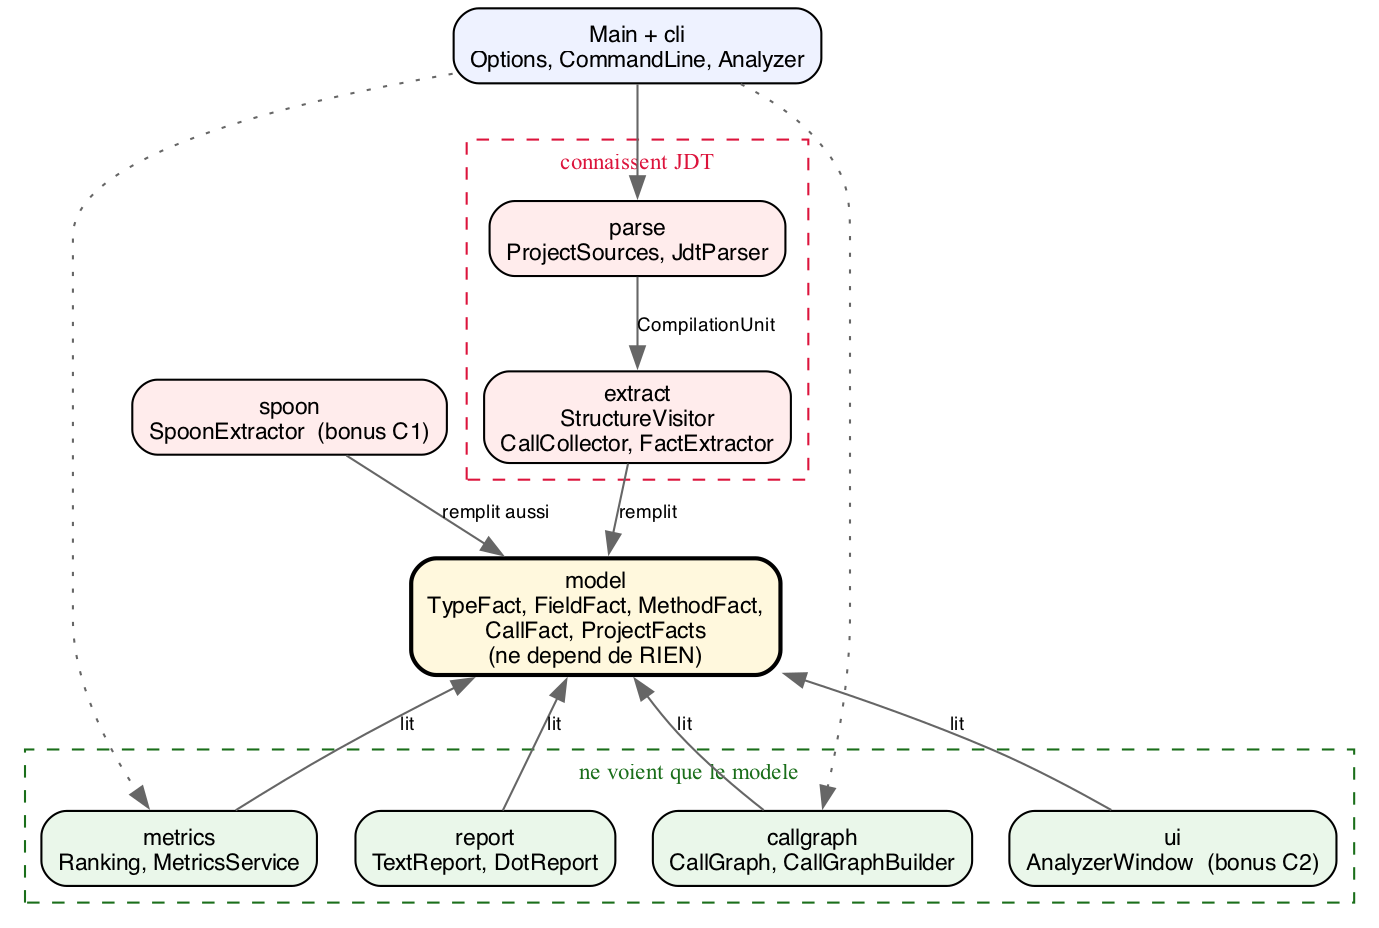
\includegraphics[width=0.9\textwidth]{images/architecture.png}
    \caption{Dépendances entre paquetages. Seuls \texttt{parse}, \texttt{extract} et \texttt{spoon} (encadré rouge) connaissent une bibliothèque d'analyse. Toutes les flèches convergent vers \texttt{model}, qui ne dépend de rien ; les traitements et les vues (encadré vert) ne lisent que lui.}
\end{figure}

\textbf{Séquence d'une analyse.} \texttt{Main} construit un \texttt{Options} ; \texttt{Analyzer} demande à \texttt{ProjectSources} la racine et les fichiers ; \texttt{JdtParser} construit les 14 \texttt{CompilationUnit} en un seul lot ; \texttt{FactExtractor} lance un \texttt{StructureVisitor} par fichier, chaque méthode déclenchant un \texttt{CallCollector} sur son corps ; les faits sont triés et assemblés ; \texttt{MetricsService} et \texttt{CallGraphBuilder} lisent ce modèle sans revenir à l'AST ; \texttt{TextReport}, \texttt{DotReport} ou \texttt{AnalyzerWindow} mettent en forme.

\section{Validation}
\label{sec:validation}

\begin{table}[H]
\centering\small
\begin{tabular}{@{}clp{7.2cm}c@{}}
\toprule
\textbf{Étape} & \textbf{Attendu} & \textbf{Obtenu} & \\
\midrule
A0 & 14 / 0 & 14 unités, 0 erreur, et 93/93 \textit{bindings} résolus & \checkmark \\
A1 & n\oe{}uds & \texttt{EnumDeclaration} sur \texttt{Category} & \checkmark \\
A2 & 15 / 59 / 21 & 15 types, 59 méthodes (9 ctors), 21 attributs & \checkmark \\
A3 & 94 / 46 / 48 / 0 & identique, et les 4 cas particuliers & \checkmark \\
B1 & déterminisme & \texttt{diff} vide sur deux exécutions & \checkmark \\
B2 & 13 métriques & toutes conformes, X = 5 et X = 4 & \checkmark \\
B3 & 59 / 44 / 46 & identique, et les 4 cas particuliers & \checkmark \\
B4 & robustesse & 3 échantillons, X mal formé refusé & \checkmark \\
\bottomrule
\end{tabular}
\caption{Tous les points de contrôle sont franchis, sans écart à expliquer. Le comportement de l'outil en dehors du projet de validation fait l'objet de la section \ref{sec:second-projet}.}
\end{table}

\subsection{Tests automatisés}

Les points de contrôle sont figés dans une suite JUnit, comme le recommande l'annexe 1. Le projet de validation et les trois échantillons de robustesse sont livrés avec le dépôt, sous \texttt{resources/}, pour que \texttt{mvn clean test} réussisse sur une copie fraîche sans dépendre de l'arborescence de nos machines. Elle nous a servi : lors de la réorganisation en paquetages puis de l'ajout de Spoon, elle a confirmé en quelques secondes qu'aucun chiffre n'avait bougé.

\begin{table}[H]
\centering\small
\begin{tabular}{@{}lcp{8.4cm}@{}}
\toprule
\textbf{Classe} & \textbf{Nb} & \textbf{Couvre} \\
\midrule
\texttt{ValidationCheckpointTest} & 13 & tous les chiffres de A0 à B3 et les cas particuliers \\
\texttt{RankingTest} & 6 & la règle des « 10 \% », \textbf{sans JDT ni fichier analysé} \\
\texttt{CommandLineTest} & 7 & chemin manquant, X = \texttt{abc}, X négatif, X absent, X = 0 \\
\texttt{RobustnessTest} & 5 & les trois échantillons, un chemin inexistant, l'ordre de validation \\
\texttt{SpoonComparisonTest} & 4 & équivalence JDT / Spoon et écarts bruts \\
\midrule
\textbf{Total} & \textbf{35} & \texttt{mvn clean test} : 0 échec \\
\bottomrule
\end{tabular}
\end{table}

\texttt{RankingTest} teste un traitement sur des données construites à la main, sans charger JDT : c'est le bénéfice concret du modèle de faits.

\subsection{Échantillons de robustesse}

Sur \texttt{missing-dep}, l'appel vers la bibliothèque absente n'a ni cible ni receveur et est signalé non résolu, tandis que \texttt{formatter.decorate}, dans la même méthode, reste résolu ; l'analyse va jusqu'au bout.

\begin{lstlisting}[language=bash]
$ java -jar target/...jar ../robustness/missing-dep --action calls
Greeter.java:3  The import org.apache cannot be resolved
Greeter.java:14 StringUtils cannot be resolved
Appels : 2 (1 internes, 0 externes, 1 non resolus)
demo.Greeter#greet(java.lang.String)
    ligne 14 : capitalize | receveur (inconnu)      | cible NON RESOLUE
    ligne 15 : decorate   | receveur demo.Formatter | cible demo.Formatter#decorate(...) [interne]
\end{lstlisting}

Sur \texttt{syntax-error}, les erreurs de \texttt{Broken.java} sont signalées, \texttt{Helper.java} est analysé normalement et l'outil ne s'arrête pas. Sur \texttt{no-java-files}, le message est explicite et le code vaut 4. Une valeur \texttt{--x abc} est refusée avec un message citant la valeur fautive et le code 2.

\subsection{Un second projet, et un chemin contenant des espaces}
\label{sec:second-projet}

Le sujet prévient que les correcteurs lanceront l'outil sur un autre projet que celui de validation. Nous avons donc fait le test nous-mêmes, un outil mis au point sur quatorze fichiers connus pouvant très bien dépendre d'eux sans qu'on s'en aperçoive.

Le projet retenu est le paquetage \texttt{gof} des exemples du patron Visiteur livrés avec l'annexe 3 (\texttt{resources/\allowbreak visitor-examples}), isolé dans un projet à part parce qu'il ne dépend d'aucune bibliothèque externe (il suffit de recopier \texttt{visitor-examples/src/gof} dans le \texttt{src} d'un dossier vide) : neuf fichiers, trois \textit{records}, deux interfaces, et une classe qui en étend une autre.

\begin{lstlisting}[language=bash]
$ java -jar target/...jar ../gof-demo --action all --x 2
Unites de compilation : 9        Erreurs de compilation : 0
Types : 9   Methodes : 19 (dont 1 constructeur)   Attributs : 1   Paquetages : 1
Appels : 40 (31 internes, 9 externes, 0 non resolus)
 1. Classes : 9      2. Lignes : 172     3. Methodes : 19    4. Paquetages : 1
 5. Methodes/classe : 2.11    6. Lignes/methode : 4.20 (63 pour 15)
 7. Attributs/classe : 0.11  13. Max parametres : 2 (TracingEvaluator#trace)
Noeuds : 19 | Arcs : 14 | Sites d'appel internes : 20 | Externes : 20
\end{lstlisting}

Aucun plantage. Les constructions absentes du projet de validation sont comptées conformément au §4.1 : les trois \textit{records} comptent pour des types, leurs accesseurs implicites ne comptent pas pour des méthodes, et la chaîne des superclasses d'un \textit{record} remonte à \texttt{java.lang.Record}. Le graphe a la forme attendue du patron Visiteur : tous les \texttt{accept} pointent vers \texttt{ExprVisitor}, et \texttt{TracingEvaluator} appelle les méthodes de \texttt{Evaluator} qu'il redéfinit.

\textbf{Un écart entre deux compteurs.} L'en-tête annonce 31 appels internes, le graphe 20 sites internes. Les onze appels manquants visent des accesseurs de \textit{record} (\texttt{Num\#value()}, \texttt{Add\#left()}. . .) : leur cible est dans le projet, mais ce n'est pas une méthode comptée, donc pas un n\oe{}ud, donc pas d'arc, et le graphe les range avec les externes. « Interne » qualifie le \textit{type} visé dans la liste des appels et la \textit{cible} dans le graphe ; les deux chiffres sont justes, les noms sont trompeurs. Le projet de validation ne contient aucun \textit{record}, ce qui explique que les deux compteurs y aient toujours donné le même résultat et que nous n'ayons rien vu. Renommer l'un des deux est la première correction que nous apporterions.

Lancé sur l'intégralité de \texttt{visitor-examples}, dont deux paquetages utilisent JDT et Spoon sans que ces bibliothèques soient sur le \textit{classpath} d'analyse, l'outil signale 118 erreurs de compilation et 80 appels non résolus, puis termine l'analyse et rend ses métriques. C'est le comportement observé sur \texttt{missing-dep}, à une autre échelle. Ce test a aussi révélé une limite que nous ignorions : \texttt{JdtParser} accepte un \textit{classpath} de JAR externes, mais \texttt{Analyzer} lui passe toujours une liste vide. Tout appel vers une bibliothèque tierce absente des sources est donc non résolu. L'exposer en option de ligne de commande serait peu coûteux.

\textbf{Chemin contenant des espaces} (demandé par B4). Le projet de validation recopié dans un dossier nommé \texttt{mon projet test} rend les mêmes 15 types, 59 méthodes, 21 attributs et 94 appels, sans guillemets particuliers sous macOS. Les chemins ne sont jamais assemblés par concaténation dans notre code : ils circulent sous forme de \texttt{java.nio.file.Path} et ne deviennent des chaînes qu'au dernier moment, dans les tableaux attendus par \texttt{setEnvironment}.

\section{Bonus : Spoon, visualisation et interface graphique}
\label{sec:bonus}

\subsection{C1 --- Refaire l'extraction avec Spoon}

\texttt{SpoonExtractor} construit un modèle Spoon et remplit \textbf{le même} modèle de faits. Le point important est ce que nous n'avons \textbf{pas} eu à faire : ni \texttt{MetricsService}, ni \texttt{CallGraphBuilder}, ni \texttt{TextReport} n'ont été modifiés.

\begin{lstlisting}[language=bash]
$ java -jar target/...jar resources/validation --action spoon
MESURE                              JDT   SPOON BRUT   SPOON (TP)
types                                15      15 / 14           15
methodes                             59      50 + 13           59
dont constructeurs                    9 13 (4 impl.)            9
attributs                            21 24 (3 const.)          21
paquetages                            4            6            4
appels                               94 107 (13 ctors)         94
\end{lstlisting}

La colonne « SPOON (TP) » coïncide avec JDT sur toutes les lignes, et le graphe issu de Spoon a les mêmes 59 n\oe{}uds, 44 arcs et 46 sites. Les écarts bruts viennent de \textbf{définitions} différentes, non d'un défaut de l'un des outils :

\begin{enumerate}
    \item \textbf{14 contre 15 types} : \texttt{getAllTypes()} ne rend que les types de premier niveau et ignore \texttt{LoanService.Loan}. Il faut \texttt{getElements(new TypeFilter<>(CtType.class))}, puis écarter les types anonymes.
    \item \textbf{50 contre 59 méthodes} : \texttt{getMethods()} exclut les constructeurs, obtenus par \texttt{CtClass.getConstructors()}. Spoon en trouve 13, dont \textbf{4 implicites} qu'il matérialise alors qu'ils ne sont pas écrits ; le sujet ne compte que les méthodes écrites, d'où le filtre \texttt{isImplicit()}.
    \item \textbf{24 contre 21 attributs} : \texttt{getFields()} inclut les \texttt{CtEnumValue}, c'est-à-dire les trois constantes de \texttt{Category}, que le §4.1 exclut.
    \item \textbf{6 contre 4 paquetages} : \texttt{getAllPackages()} compte le paquetage racine et \texttt{library}, qui ne contient directement aucune classe.
    \item \textbf{107 contre 94 appels} : Spoon représente \texttt{super(...)} et \texttt{this(...)} par des \texttt{CtInvocation}, au même titre qu'un appel ordinaire. Avec JDT ce sont des n\oe{}uds d'un type différent, qu'on ne risque pas de confondre.
\end{enumerate}

Spoon épargne du code, mais c'est ce confort qui masque les questions de définition que le TP pose. Mise en garde vérifiée : en mode \textit{noClasspath}, il attribue \texttt{capitalize} à \texttt{org.apache.commons.lang3.StringUtils} en le déduisant de l'\texttt{import} alors que la bibliothèque est absente ; il ne faut donc pas conclure qu'un appel est résolu sans l'avoir vérifié.

\subsection{C2 --- Visualisation et interface graphique}

L'option \texttt{--dot} écrit le graphe au format Graphviz, les n\oe{}uds groupés par classe et les étiquettes raccourcies en \texttt{methode/arite}. Le filtre \texttt{--dot-package} est indispensable en pratique : sur 59 n\oe{}uds l'image devient dense.

\begin{figure}[H]
    \centering
    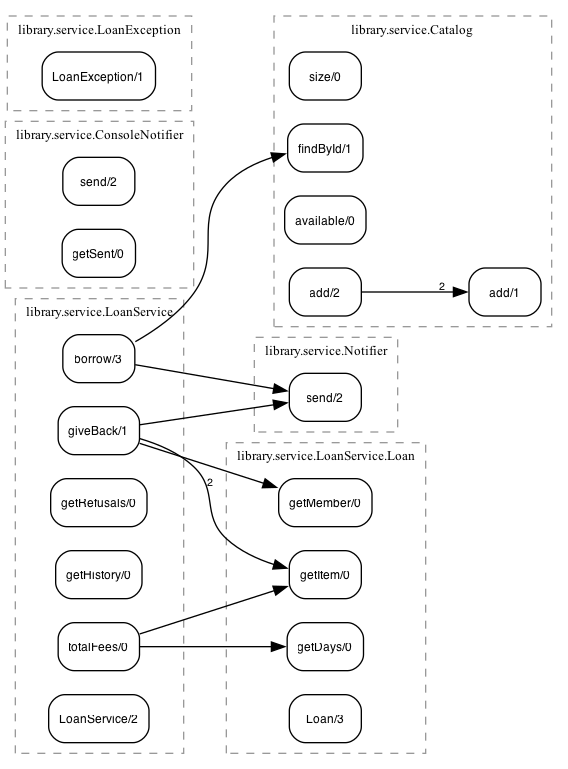
\includegraphics[width=0.58\textwidth]{images/graphe-service.png}
    \caption{Graphe du paquetage \texttt{library.service} (Graphviz 14.1.0). L'arc \texttt{add/2} $\rightarrow$ \texttt{add/1} porte le poids 2, conformément au point de contrôle B3.}
\end{figure}

L'option \texttt{--gui} ouvre une fenêtre Swing. Conformément au sujet, ce n'est qu'une \textbf{seconde façon d'afficher les résultats du même modèle} : elle appelle les mêmes composants que la ligne de commande et ne calcule rien. Quatre onglets, un par étape : Structure, Appels, Métriques avec réglage du seuil X, et Graphe d'appel avec interrogation dans les deux sens.

\begin{figure}[H]
    \centering
    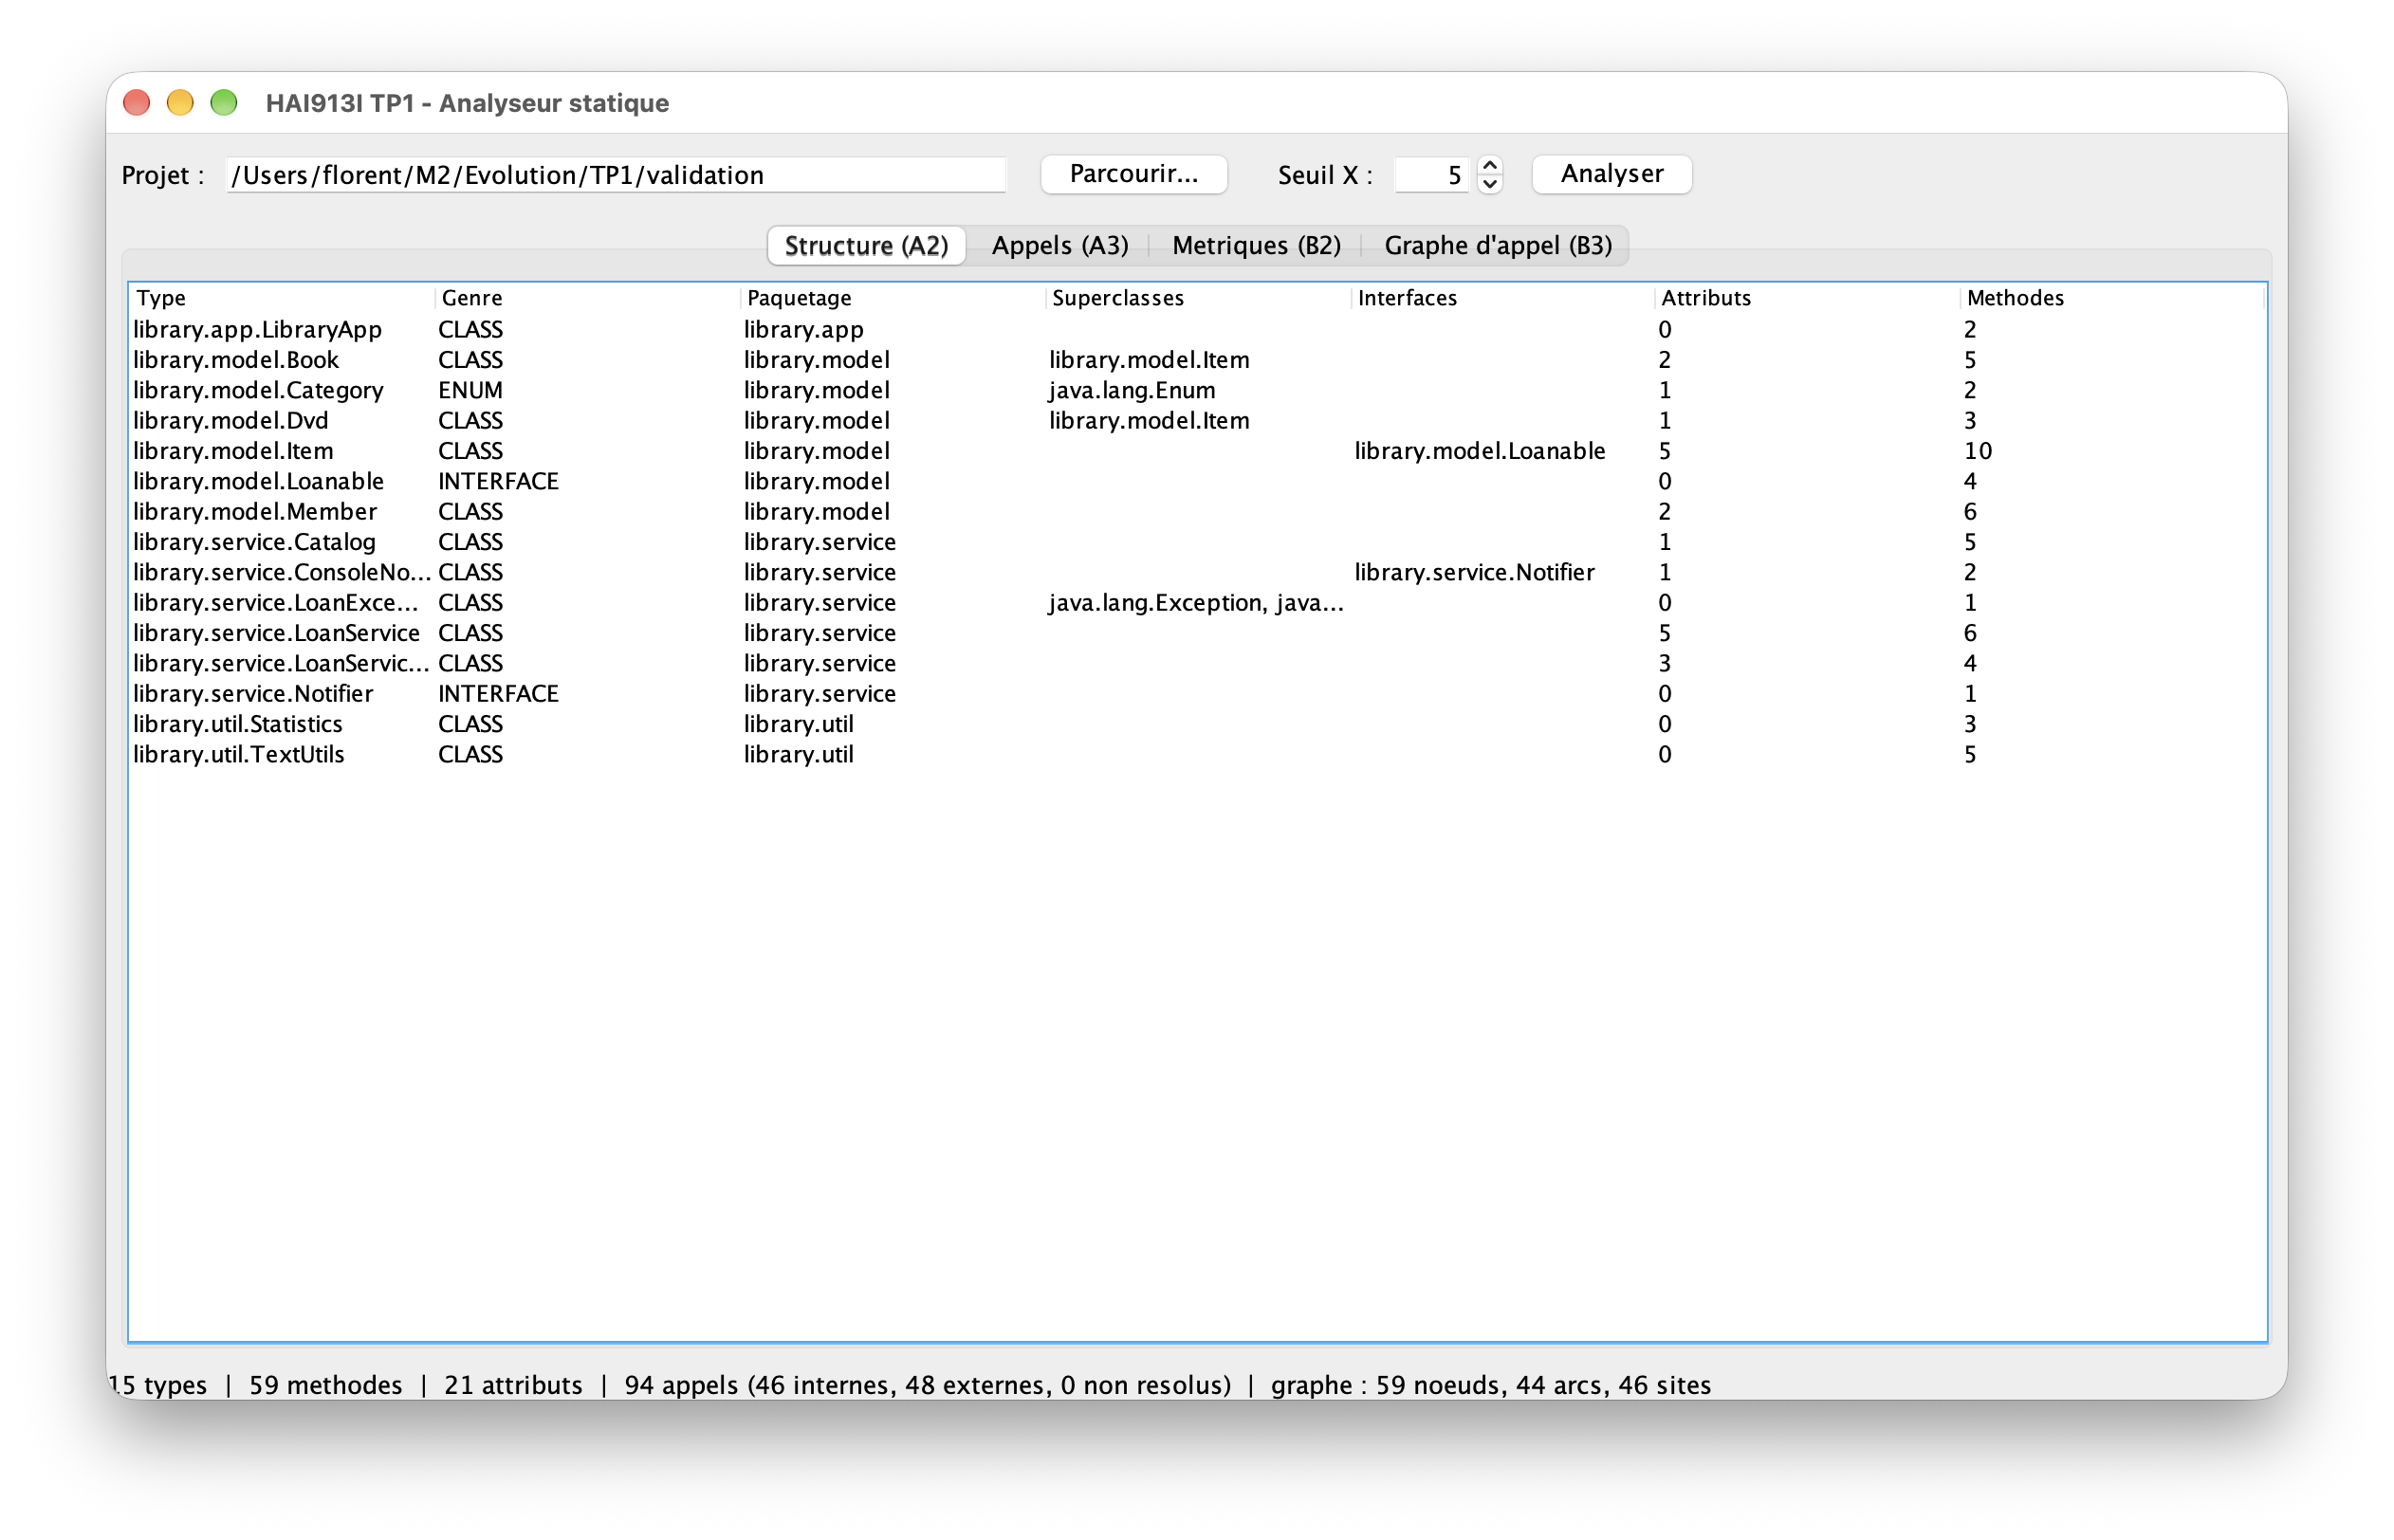
\includegraphics[width=0.85\textwidth]{images/gui-structure.png}
    \caption{Onglet « Structure (A2) ». \texttt{LoanService} et sa classe membre \texttt{LoanService.Loan} occupent deux lignes distinctes (6/5 et 4/3), et \texttt{Category} apparaît avec le genre \texttt{ENUM}.}
\end{figure}

\begin{figure}[H]
    \centering
    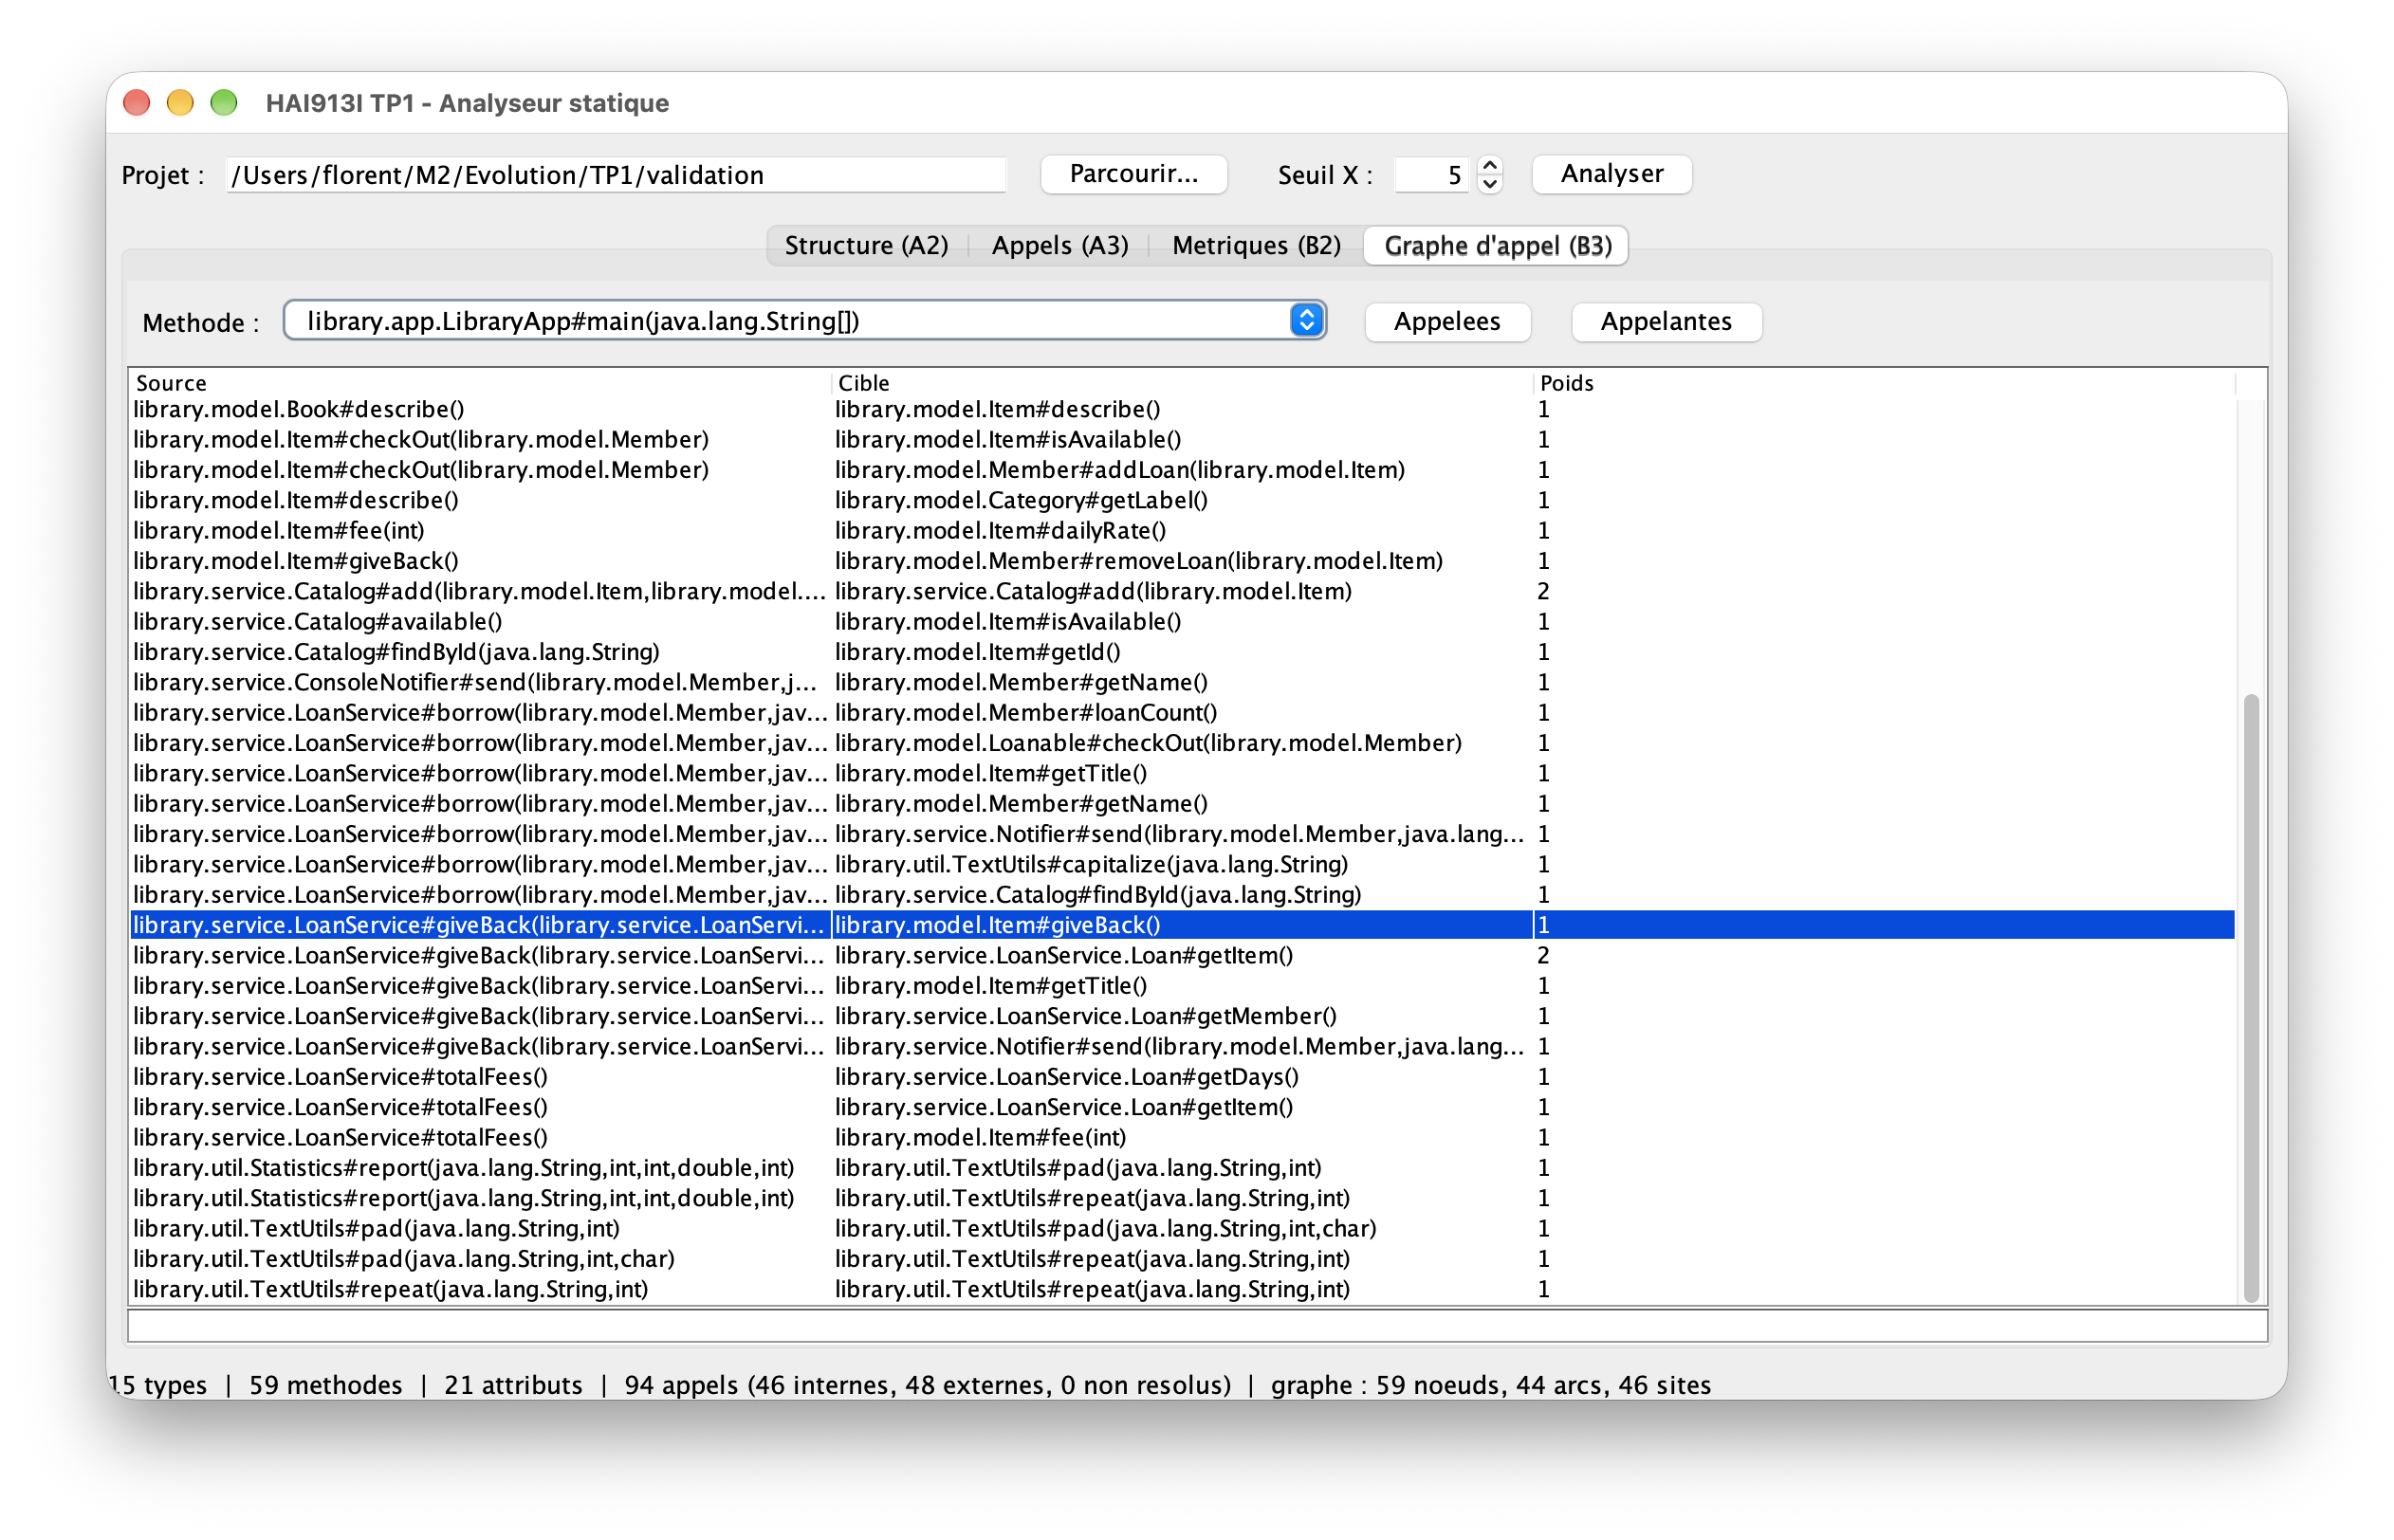
\includegraphics[width=0.85\textwidth]{images/gui-graphe.png}
    \caption{Onglet « Graphe d'appel (B3) ». La seule valeur de poids supérieure à 1 est l'arc \texttt{Catalog\#add(Item,Item)} $\rightarrow$ \texttt{Catalog\#add(Item)} ; la dernière ligne, \texttt{TextUtils\#repeat} vers lui-même, matérialise la récursion.}
\end{figure}

\subsection{C3 --- Analyser un projet de taille moyenne}

Le projet analysé est notre propre analyseur : 29 fichiers, 2 109 lignes, 10 paquetages, soit environ quatre fois le projet de validation. Le choix n'est pas seulement commode. Le rapport affirme depuis la section \ref{sec:architecture} que le modèle de faits est un point d'arrivée dont rien ne repart ; faire mesurer cette affirmation par l'outil lui-même la transforme en fait vérifiable.

\begin{lstlisting}[language=bash]
$ java -jar target/hai913i-tp1-analyzer.jar . --action all --x 5
Unites de compilation : 29       Erreurs de compilation : 213
Types : 30   Methodes : 128 (dont 15 constructeurs)   Attributs : 28   Paquetages : 10
Appels : 1040 (318 internes, 476 externes, 246 non resolus)
 2. Lignes : 2109    5. Methodes/classe : 4.27    6. Lignes/methode : 10.35 (1325 pour 128)
 7. Attributs/classe : 0.93
 8. plus de methodes  : [StructureVisitor, SpoonExtractor, TextReport, AnalyzerWindow]
 9. plus d'attributs  : [AnalyzerWindow, Analyzer, CallCollector]
10. intersection      : [AnalyzerWindow]
Noeuds : 128 | Arcs : 145 | Sites internes : 180 | Externes : 614 | Non resolus : 246
\end{lstlisting}

\textbf{Ce que le graphe révèle, et que nous ne pouvions pas affirmer autrement.} Le paquetage \texttt{model} reçoit 29 arcs et n'en émet que 4, et ces quatre-là sont internes à \texttt{ProjectFacts} : \texttt{callCount}, \texttt{internalCallCount}, \texttt{externalCallCount} et \texttt{unresolvedCallCount} appellent toutes \texttt{calls()}. Le modèle de faits est donc bien un puits au sens du graphe d'appel : tout le monde l'appelle, il n'appelle personne. C'est la traduction mesurée de la frontière décrite en section 2.1, et c'est la propriété qui a permis de brancher Spoon puis l'interface graphique sans toucher aux traitements.

\textbf{Ce que les métriques révèlent, et qui nous dérange.} La question 10 désigne \texttt{AnalyzerWindow} comme seule classe à la fois dans les 10 \% les plus fournies en méthodes et en attributs. Le diagnostic est correct sans être inquiétant : une fenêtre Swing accumule des composants en attributs, et notre interface ne calcule rien. La question 12 est plus gênante pour nous : la méthode la plus longue de \texttt{Analyzer} est \texttt{run}, avec 83 lignes. Notre propre rapport reproche au « \textit{main} de mille lignes » de ne pas être une architecture ; notre chef d'orchestre est sur la même pente, et devrait être découpé par action.

Le contraste des moyennes mérite aussi d'être noté : 10,35 lignes par méthode ici contre 4,64 sur le projet de validation. Le projet de validation est un jeu d'essai, pas un logiciel ; en tirer des seuils que l'on appliquerait à du code réel n'aurait aucun sens, ce qui illustre concrètement la mise en garde du CM 01 sur ce qu'une métrique permet ou non d'affirmer.

\textbf{Les limites que cette analyse expose.} 246 appels sur 1 040, soit 24 \%, sont non résolus, et 213 erreurs de compilation sont signalées. Toutes ont la même origine : notre analyseur dépend de JDT et de Spoon, et ces bibliothèques ne sont pas sur le \textit{classpath} d'analyse puisque nous n'exposons pas d'option pour les y mettre (section \ref{sec:second-projet}). Le graphe obtenu reste exploitable, puisque les 318 appels internes sont tous résolus, mais l'expérience chiffre le coût de cette limite sur un projet réaliste : un quart des appels invisibles. Sur un projet à dépendances lourdes, la proportion serait pire encore, et c'est la première raison pour laquelle nous exposerions un \textit{classpath} avant toute autre amélioration.

\section{Difficultés rencontrées}

\textbf{Les deux classes \texttt{Path}.} La première erreur de compilation venait d'un import automatique de l'IDE : \texttt{org.eclipse.core.runtime.Path} au lieu de \texttt{java.nio.file.Path}. JDT tire une vingtaine de bibliothèques Eclipse dont plusieurs classes portent le nom de classes du JDK, et le symptôme (\texttt{cannot find symbol: method of(String)}) ne pointe pas vers l'import fautif.

\textbf{Un SDK invalide dans l'IDE.} IntelliJ affichait 45 erreurs dans un fichier n'utilisant que des classes du JDK, alors que \texttt{mvn clean compile} passait : le SDK déclaré avait un \textit{classpath} vide, si bien que même \texttt{java.io.IOException} était inconnu. La leçon dépasse l'anecdote : quand l'IDE et la ligne de commande se contredisent, c'est la ligne de commande qui fait foi, puisque c'est \texttt{mvn} qui produit le livrable.

\textbf{L'attribution des appels dans les lambdas.} La subtilité qui a demandé le plus de réflexion est la différence de traitement entre A2 et A3 : les types des lambdas et classes anonymes ne comptent pas, ce qui invite à les élaguer, mais les appels qu'elles contiennent doivent être attribués à la méthode englobante. Le même élagage dans les deux visiteurs nous aurait donné 93 appels au lieu de 94.

\textbf{Parties incomplètes.} Toutes les étapes A0 à B4 sont franchies, ainsi que les trois bonus. Deux imperfections connues subsistent, l'une et l'autre repérées en analysant des projets extérieurs (sections \ref{sec:second-projet} et \ref{sec:bonus}) : l'étiquette « interne » de la liste des appels et le compteur de sites internes du graphe ne recouvrent pas la même notion en présence de \textit{records} ; et le \textit{classpath} de JAR externes, prévu dans \texttt{JdtParser}, n'est exposé nulle part sur la ligne de commande, ce qui laisse 24 \% des appels non résolus sur un projet à dépendances. Nous les documentons plutôt que de les corriger dans l'urgence ; la seconde est notre première priorité.

Un défaut repéré de la même façon a en revanche été corrigé : l'ordre de validation des arguments, décrit en B4, qui faisait répondre « le seuil X est obligatoire » à un utilisateur ayant simplement mal tapé son chemin.

\section{Utilisation des outils d'intelligence artificielle}

Dans le cadre de ce projet, nous avons utilisé l'assistant \textbf{Claude} lors de sessions interactives pour nous accompagner sur différentes tâches. Ses interventions ont porté sur l'analyse et la compréhension du sujet, la réalisation de l'interface graphique, l'écriture de tests JUnit pour valider notre code, ainsi que sur la rédaction et la relecture de ce rapport.
\textbf{Trois exemples représentatifs de l'aide obtenue.}

\begin{itemize}
\item \textit{Diagnostic.} Notre première erreur de compilation, \texttt{cannot find symbol: method of(String)} sur \texttt{Path}, ne désignait pas sa cause. L'hypothèse de l'import automatique erroné (\texttt{org.eclipse.core.runtime.Path} au lieu de \texttt{java.nio.file.Path}) vient de l'assistant ; nous l'avons confirmée en relisant la ligne d'import.
\item \textit{Explication de cours.} La distinction entre \texttt{EnumDeclaration} et \texttt{TypeDeclaration}, qui descendent toutes deux d'\texttt{AbstractTypeDeclaration} sans descendre l'une de l'autre, nous a été expliquée alors que notre visiteur comptait 14 types. Vérification dans la Javadoc de JDT, puis sur le comptage, passé à 15.
\item \textit{Conception.} Nous avons discuté des formes possibles pour les identifiants de méthode avant de retenir la chaîne textuelle à types effacés. L'échange a servi à écarter les représentations fondées sur un objet JDT, qui auraient fait entrer la bibliothèque d'analyse dans le modèle de faits et rendu l'extraction Spoon impossible à brancher.
\end{itemize}

\section{Regard critique}
\label{sec:critique}

\textbf{Les appels virtuels} sont la limite la plus importante, et elle est visible dans nos propres chiffres : \texttt{Item\#checkOut(Member)} n'a aucune appelante dans notre graphe alors qu'elle est exécutée à chaque emprunt. L'appel est écrit \texttt{loanable.checkOut(member)}, le type déclaré est l'interface, et l'arc vise donc \texttt{Loanable\#checkOut}. Un développeur qui utiliserait ce graphe pour évaluer l'impact d'une modification de \texttt{Item.checkOut} conclurait à tort que personne ne l'appelle. Une analyse CHA ajouterait les arcs vers les redéfinitions connues, mais introduirait des arcs jamais empruntés : il n'y a pas de bonne réponse, seulement un compromis entre faux négatifs et faux positifs, qu'il faut documenter.

\textbf{Réflexion, proxys, injection} sont invisibles : notre analyse ne voit que ce qui est écrit. Sur une application utilisant un conteneur d'injection, une part significative du graphe réel échapperait à l'outil. De même, 48 des 94 appels sortent du projet : nous les comptons sans y descendre, si bien que le graphe décrit la structure interne, pas le comportement complet.

\textbf{Pertinence des métriques.} Les treize métriques mesurent la taille et la répartition, et désignent correctement \texttt{Item} et \texttt{LoanService} comme les deux classes centrales. Leurs angles morts méritent d'être signalés : les lignes de code ne mesurent pas la complexité, une méthode de 14 lignes avec trois conditions imbriquées étant plus difficile à faire évoluer qu'une méthode de 30 lignes linéaires ; la moyenne de 3,93 masque qu'\texttt{Item} a 10 méthodes quand d'autres en ont 2 ; le seuil des « 10 \% » est arbitraire et très sensible sur 15 classes, où $k = 2$ ; enfin aucune métrique de \textbf{couplage} n'est demandée, alors que c'est elle qui prédit le mieux la difficulté d'évolution. C'est l'objet du TP 2, et c'est pourquoi nous avons conservé le poids des arcs bien que le TP 1 ne l'exploite pas.

\textbf{Ce que nous améliorerions}, par ordre de priorité : distinguer nominalement les deux compteurs d'appels internes (section \ref{sec:second-projet}) ; exposer un \textit{classpath} de JAR externes sur la ligne de commande, pour qu'un projet à dépendances ne soit plus analysé à moitié ; ajouter une option CHA et mesurer le nombre d'arcs qu'elle ajoute ; produire un export JSON consommable par le TP 2 ; calculer une complexité cyclomatique en complément de la question 6, le nombre de lignes n'en étant qu'une approximation grossière.

\section{Conclusion}

L'outil franchit l'ensemble des points de contrôle, de A0 à B4, sans écart sur le projet de validation, et les bonus C1 et C2 sont traités.

Deux points nous semblent valoir d'être retenus.

La frontière entre la bibliothèque d'analyse et les traitements nous a d'abord coûté du travail : il a fallu définir un modèle intermédiaire là où l'on pouvait calculer directement sur l'AST. Le bénéfice est apparu ensuite, et le cas le plus net est le bonus C1 : brancher Spoon s'est réduit à écrire un second extracteur, les treize métriques et le graphe fonctionnant sans modification.

La validation, ensuite. Les chiffres attendus fournis par le sujet constituent un filet très efficace, mais ils ne couvrent que les constructions présentes dans le projet de validation. Celui-ci ne contient pas de \textit{record} ; neuf fichiers supplémentaires ont suffi à faire apparaître la divergence de compteurs décrite en section \ref{sec:second-projet}, présente depuis le début et invisible jusque-là.

Le graphe produit, et en particulier le poids de ses arcs, constitue la donnée d'entrée du calcul de couplage du TP 2.

\section*{Annexe --- Environnement et lancement}
\addcontentsline{toc}{section}{Annexe --- Environnement et lancement}

JDK OpenJDK 17.0.16, Maven 3.9.11, Eclipse JDT Core 3.46.0, Spoon 11.5.0, JUnit Jupiter 5.14.4, Graphviz 14.1.0, macOS 26.6 (Apple Silicon), IntelliJ IDEA 2026.2.

\begin{lstlisting}[language=bash]
cd hai913i-tp1-analyzer
mvn clean package
java -jar target/hai913i-tp1-analyzer.jar resources/validation --x 5
\end{lstlisting}

Dépôt Git : \url{https://github.com/AdrienSmbr/TP1-HAI913I} \\
Vidéo de démonstration : \textcolor{red}{\texttt{[URL à compléter]}}

\section*{Références}
\addcontentsline{toc}{section}{Références}

\begin{enumerate}
    \item Bachar Rima, \textit{HAI913I --- TP 1 : Analyse statique} et ses annexes 1, 2 et 3, Université de Montpellier, 2026--2027.
    \item Cours HAI913I, CM 01 et CM 02.
    \item Javadoc Eclipse JDT Core (\texttt{ASTParser}, \texttt{ASTVisitor}, \texttt{CompilationUnit}) et guide \textit{Manipulating Java code}. \url{https://help.eclipse.org/latest/}
    \item Documentation de Spoon. \url{https://spoon.gforge.inria.fr}
    \item R. Pawlak \textit{et al.}, « Spoon: A Library for Implementing Analyses and Transformations of Java Source Code », \textit{Software: Practice and Experience}, 2015.
    \item E. Gamma \textit{et al.}, \textit{Design Patterns}, Addison-Wesley, 1994 (patrons Visiteur et Façade).
    \item Documentation Graphviz, format DOT. \url{https://graphviz.org/doc/info/lang.html}
\end{enumerate}

\end{document}
